\section{OSI Referenzmodell}
    \begin{highlight}{Klassifizierung von Diensten}
    \begin{center}
        \begin{minipage}{0.46\linewidth}
                \tcbsubtitle{Verbindungsorientiert}
                    \begin{itemize}
                        \item Verbindungsaufbau nötig
                        \item Informationen vom Empfänger - Optionen aushandeln
                        \item Reihenfolge der Daten bleibt erhalten
                    \end{itemize}
                \tcbsubtitle{Verbindungslos}
                \begin{itemize}
                    \item Jederzeit (send and forget)
                    \item Ziel muss nicht bereit sein
                    \item einfacher umzusetzen
                \end{itemize}
        \end{minipage}
        \hfill\vline\hfill
        \begin{minipage}{0.47\linewidth}
            \tcbsubtitle{Zuverlässig}
                \begin{itemize}
                    \item Kein Datenverlust
                    \item Sicherung durch Fehler-Erkennung/-Korrektur
                    \item Text-Nachrichten
                \end{itemize}
            \tcbsubtitle{Unzuverlässig}
            \begin{itemize}
                \item Möglicher Datenverlust
                \item Keine Sicherung
                \item Streaming
            \end{itemize}
        \end{minipage}
    \end{center}
\end{highlight}

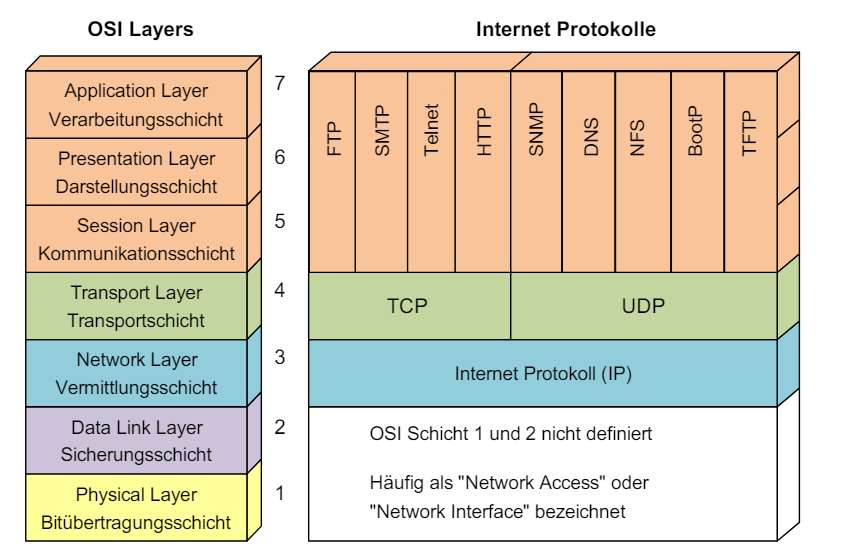
\includegraphics[width=1\linewidth]{images/OSI_Modell.png}




 
    
 